\documentclass{article}

%package setup
\usepackage{graphicx}
\usepackage{amsmath}
\usepackage{fancyhdr}
\usepackage[margin=1in]{geometry}
\usepackage{comment}
\usepackage{placeins}
\usepackage{parskip}
\usepackage{subcaption}
\usepackage{appendix}
\usepackage{soul}
\usepackage{comment}
\usepackage[hidelinks]{hyperref}
\usepackage{matlab-prettifier}
\usepackage{minted}
\usepackage{enumitem}
\usepackage{float}
\usepackage{textcomp, gensymb}

\pagestyle{fancy}
\fancyhf{} % Clear header/footer settings
\rhead{\thepage} % Page number on the right in the header
\lhead{ASE375 Lab Report 2} % Your lab report title on the left

\begin{document}

\begin{titlepage}
  \centering
  
\includegraphics[width=10cm]{ase-logo-formal.png}  % Adjust the width as needed
  \vspace{1cm}  % Add some vertical space
 
  \Large \textbf{ASE 375 Electromechanical Systems}\\
  \large \textbf{Section 14115}\\
  \vspace{0.5cm}
  \textbf{Monday: 3:00 - 6:00 pm}\\
 
  \vspace{1cm}
 
  \hrule
  \vspace{0.5cm}
 
  \Huge \textbf{Report 2:\\
  Temperature Sensor Measurements}\\
  \Huge \textbf{}\\
 
  \vspace{0.5cm}
  \hrule
 
  \vspace{1cm}
 
  \normalsize \textbf{Andrew Doty, Andres Suniaga, Dennis Hom}\\
  \normalsize \textbf{Due Date: 02/12/2024}
 
\end{titlepage}
\newpage

\tableofcontents
\thispagestyle{empty}
\newpage

\section{Introduction}
This experiment consisted of measuring temperature with three different sensors: a Thermocouple, Thermistor, and an Integrated Circuit Temperature sensor. Data collection was made possible through a Data Acquisition (DAQ) system used to process the different temperature measurements in LabVIEW, a graphical interface that modeled the temperature sensors' measurements in real-time. 

The purpose of this experiment was to learn how to simulate our data through LabVIEW along with observing and understanding the behaviour of the three temperature sensors in different environments: $(1)$ at room temperature, $(2)$ in water near freezing conditions, and $(3)$ in water closer to boiling conditions. 

\section{Equipment}
The equipment used in this experiment include the following:  

K-type Thermocouple:  Temperature sensor with two different metals joined together at one end.  A K-type thermocouple uses Chromel-Alumel metals.  It will be connected to the DAQ via the NI 9211 thermocouple input module.  

SA1-TH Series Thermistor:  Temperature sensor that measures electrical resistance as a response to a change in temperature.  It is connected to the NI 9215 via breadboard in its own circuit with $1\text{k}\Omega$ resistor.
\begin{figure}[H]
    \centering
    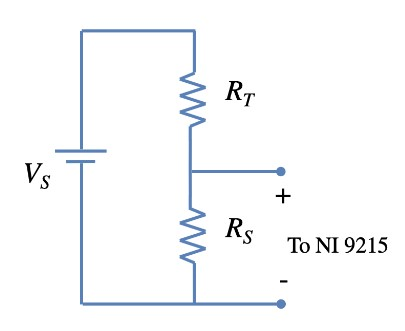
\includegraphics[width=0.25\textwidth]{lab2images/thermistor_circuit.jpg}
    \caption{Thermistor Circuit}
\end{figure}

TMP36 Temperature Sensor: Analog low voltage sensor.  It is connected to the NI 9215 via the breadboard.  

Breadboard: a reusable solderless prototyping board used for building electronic circuits. Components are inserted into interconnected rows and columns of holes, allowing for easy and temporary assembly of circuits for testing and experimentation.

Circuit Components:  various length male-to-male jumper wires, $1\text{k}\Omega$ resistor, 5V power supply.

DAQ:  Data Aquisition system that digitizes analog information into "bins" for a computer.  The specific DAQ had two units, the NI 9215 and NI 9211.  Specific Datasheets for each are included in the appendices.  

Thermometer:  Regular mercury thermometer, using change in volume as a response to a change in temperature.  Used to measure true temperature with 0.5 degrees least count.  

Water:  Access to water at two temperatures, near boiling, and ice cold. 

\section{Procedure}
\begin{figure}[H]
\centering
\includegraphics[width=0.5\textwidth, angle = -90]{lab2images/circuit_board_mug_and_sensors.jpg}
\caption{Temperature Sensors, Water mug, and Breadboard circuit}
\end{figure}

The DAQ, with the NI 9211 and NI 9215 modules already installed, was connected to an external 5V power supply as well as to the computer.  The LabVIEW software is used to digitize the data from the temperature sensors.  To do this, the following block diagram was created.

\begin{figure}[H]
\centering
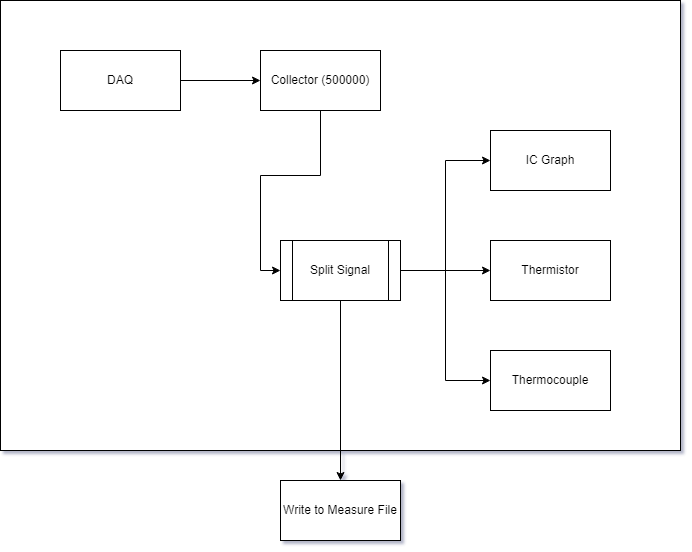
\includegraphics[width=0.5\textwidth]{lab2images/ProcessDiagram.png}
\caption{Process Diagram}
\end{figure}

\begin{figure}[H]
    \centering
    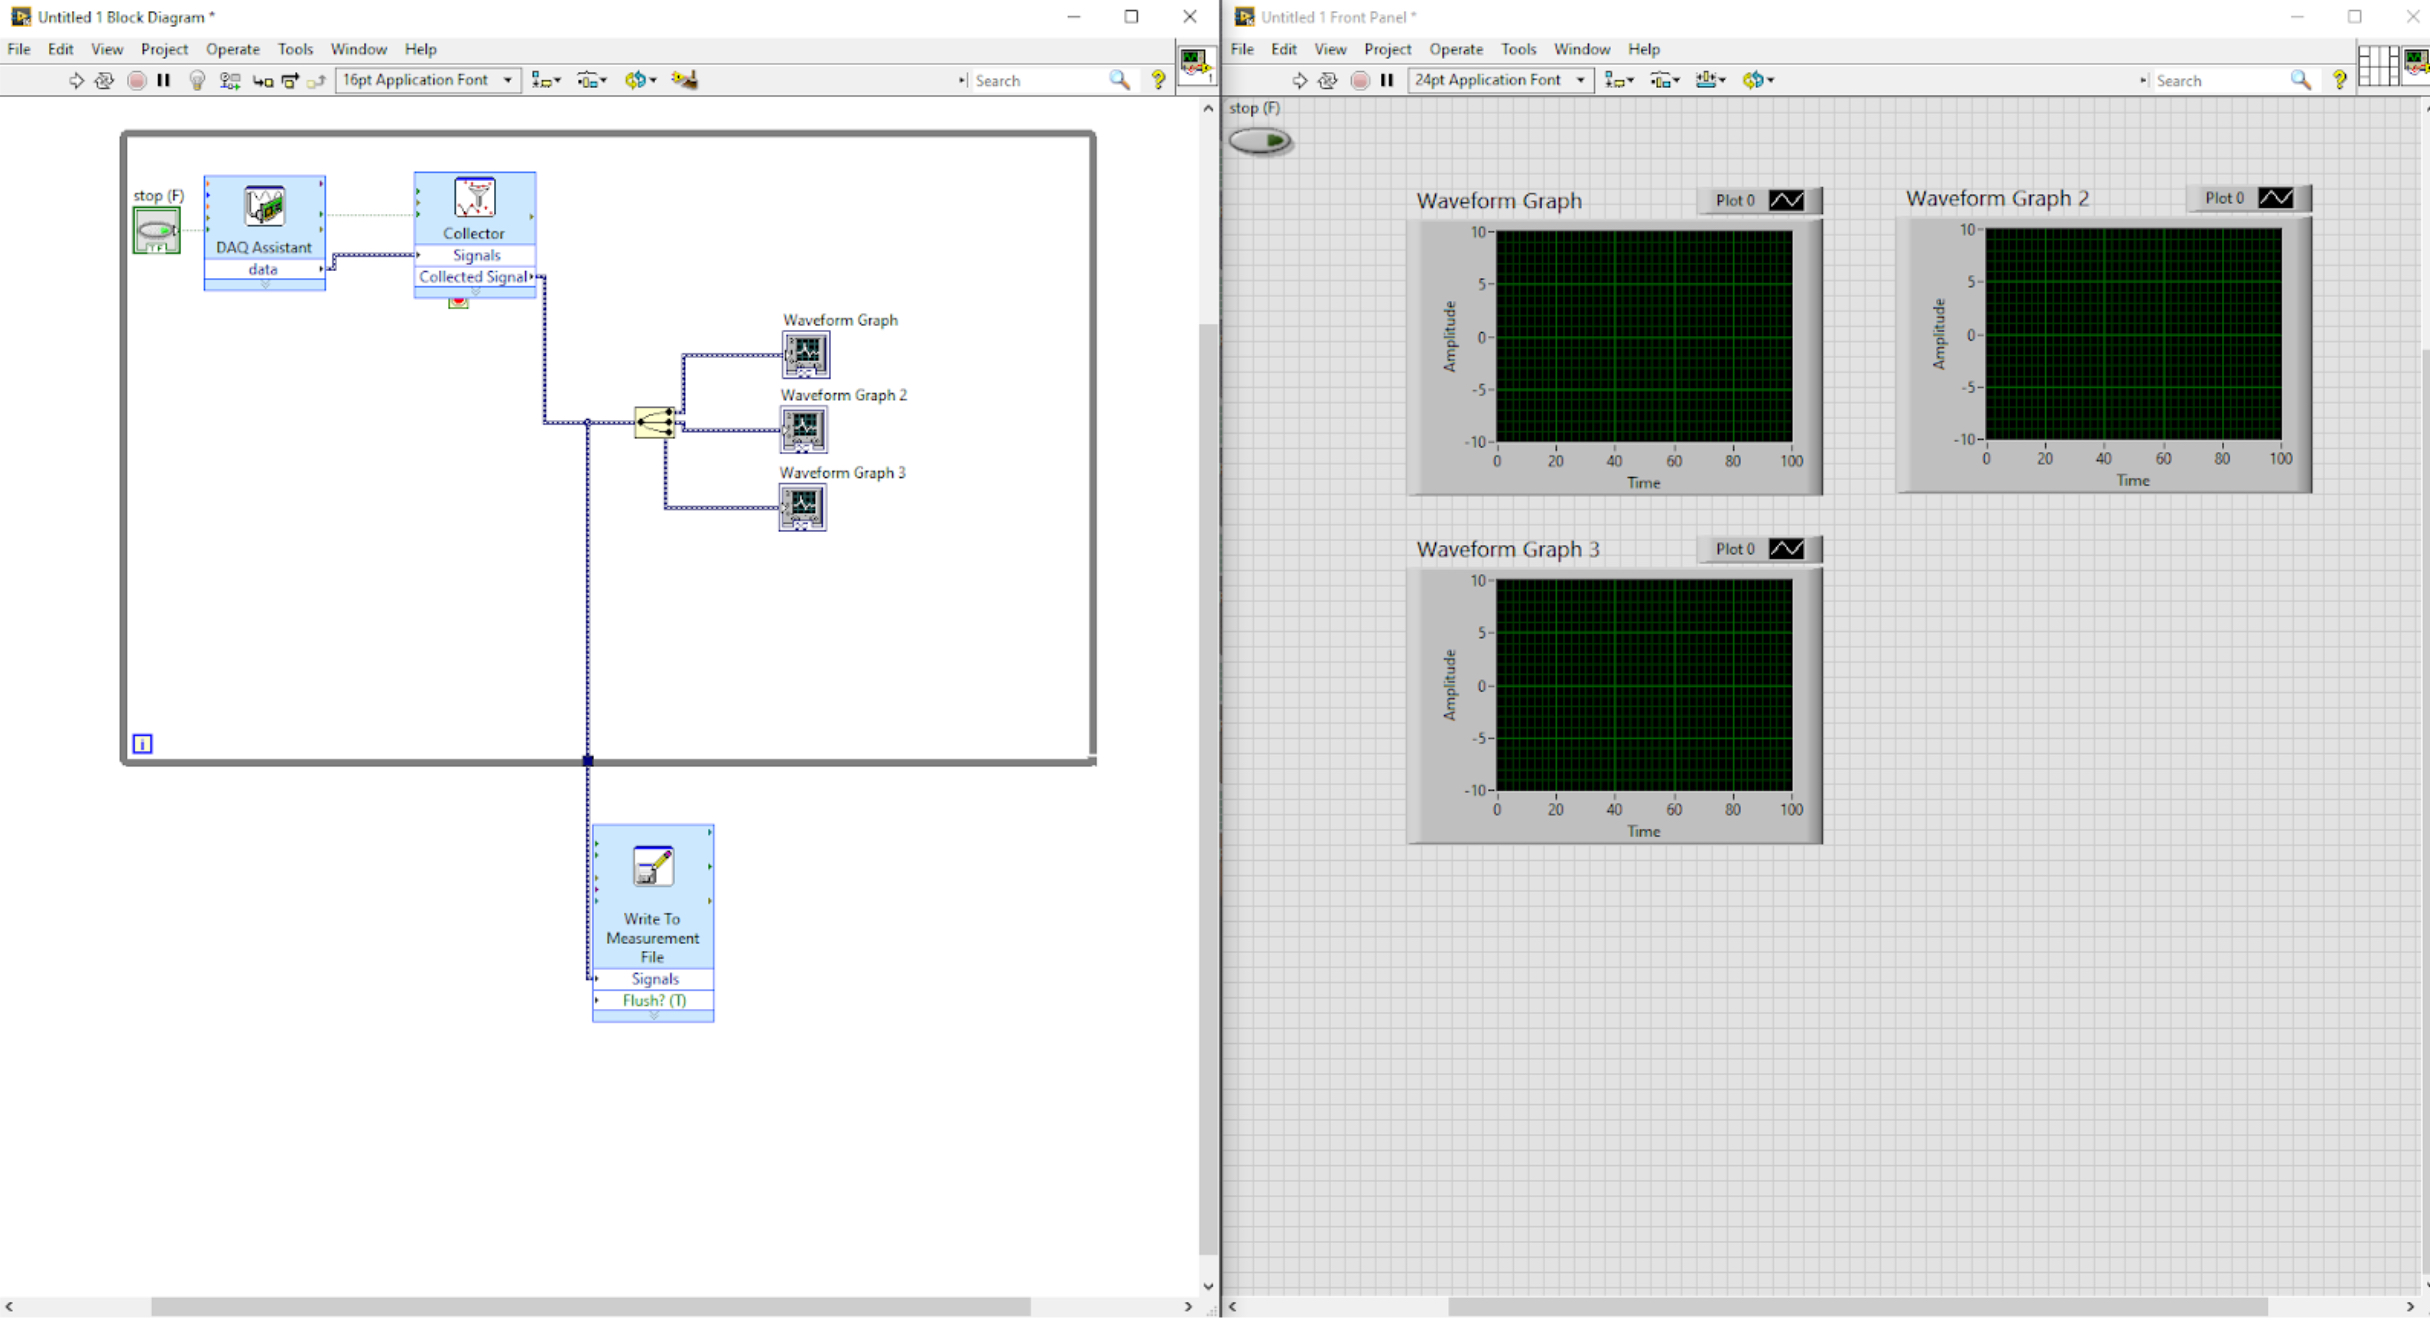
\includegraphics[width=0.5\textwidth]{lab2images/68154.jpg}
    \caption{Process Diagram screenshot}
    \end{figure}

The DAQ block had signals for each sensor, measuring at a 1000hz frequency.  The collector is initially given a size of 500,000 samples.  Each sensor from the DAQ was given its own graph using a split signal, and a "write to measure file" block was placed to save our data to an Excel file.  

Now that our digital sensing was set up, we had to create the physical circuits. The thermocouple was connected directly into the NI 9211 module.  The NI 9215 and power supply were connected to a breadboard. 
 The Thermistor was connected to a $1\text{k}\Omega$ resistor in a voltage divider configuration. The TMP36 was connected to the 5V power supply and the NI 9215 module.  This configuration is shown in figure 2.

 Additionally, for each part of this experiment, the true temperature was measured via a mercury thermometer.

\subsection{Part 1} % Subsection 1

To gather the room temperature data, the sensors were placed in an unused area in the lab room and left to sit for a few minutes without anyone moving near them or touching them.  This was to stop heat from diffusing through the rubber casing of the wire or through the air. The LabVIEW simulation was run for 3 minutes at 1000hz and the data was saved to the Excel file. The results of the simulation are shown in the figures below.

\subsection{Part 2} % Subsection 2
 
\subsubsection{Part 2a: Hot Water} % Subsubsection 1

An electric kettle was used to heat up water to near boiling.  The LabVIEW simulation was started with the sensors in the ambient environment until the graphs appeared to reach steady-state, which acts as an asymptote on the value from the sensors, and then were abruptly submerged in the boiling water.  They stayed in the water until the graph once again appeared at steady-state.  This experiment was run over 2 minutes and at a frequency of 1000hz.  The region between the two steady-states will be used to calculate the time-constant.  

\subsubsection{Part 2b: Water Cooling} % Subsubsection 2

For this part of the experiment, the collector block's size was changed to one million samples to account for the amount of time it would take for the water to cool from its initial boiling state to a safe and drinkable condition.  At a frequency of 1000hz, this gave us approximately 16 minutes of data collection.  The sensors were placed in the boiling water and the data was collected until the true temperature, measured via a thermometer, was at \(40^\circ C\), as that is the optimal temperature for safe drinking water.  

\subsubsection{Part 2c: Ice-Hot} % Subsubsection 3

Place the three sensors in a bowl of ice-cold water, wait for the graphs to reach equilibrium, and then quickly take them out of the ice water, and into the hot water, measuring until it reaches steady-state.  The region between the equilibrium in ice water and the equilibrium in hot water is the time constant we are measuring.  In our experiment, the ice water was at \(40^\circ C\) and the hot water was at \(87^\circ C\).  

\subsubsection{Part 2d: Quick Changes} % Subsubsection 4

Lastly, after the sensor had reached steady state in the water above, we took the sensors out of the water and measured the time it takes for the sensors to return to room temperature. We saved the data to an Excel file with a frequency of 1000 hz. 

\subsubsection{Part 2e: Sensor Repetition} % Subsubsection 5

The data was measured simultaneously for each sensor.  

\section{Data Processing}
\subsubsection*{Variables}
\begin{enumerate}[label = \roman*.]
    \item \(N = \) Number of Samples
    \item \(f_{s} = \) Sampling Frequency, $s^{-1}$
    \item \(\Delta t_{s} = \) Sampling Interval, $s$
    \item \(\gamma = \) Confidence Level, \%
    \item \(R_{S} = \) Sensor Resistance, Ohms = $\Omega$ (In this experiment it will be $1\text{k}\Omega$)
    \item \(V_{S} = \) Source voltage, Volts = $V$ ($5\;V$ for this experiment)
    \item \(R_{T} = \) Themistor resistance, $\Omega$
\end{enumerate}

\subsubsection*{Equations}
\begin{enumerate}[label = \Roman*.]
    \item Sample Mean: \(\bar{x} = \dfrac{1}{N}\displaystyle\sum_{i=1}^{N} x_{i}\) 
    \item Standard Deviation of finite $N$, normalized by $N-1$: \(S_{x} = \sqrt{\displaystyle\sum_{i=1}^{N} \dfrac{(x_{i} - \bar{x})^{2}}{N-1}}\)
    \item Standard Deviation of the Mean: \(\dfrac{S_{x}}{\sqrt{N}}\)
    \item Average Measurement w/ Confidence Interval: \(\bar{x} \pm t_{stat}\cdot \dfrac{S_{x}}{\sqrt{N}}\)
    \item \textit{Steinhart-Hart Relation}: \(\dfrac{1}{T} = A + B\cdot ln(R_{T}) + C\cdot (ln(R_{T}))^{3}\), where $A$, $B$, $C$ are the Thermistor's calibration coefficients.
\end{enumerate}  

\subsection*{Conversions}
The IC/TMP36 sensor originally outputs voltage. This was converted to $\degree C$ by taking the IC TMP36 output, say $x_{V}$ ($V$ for volt), and converting by $x_{\degree C} = 100\cdot(x_{V}-0.5)$. This conversion comes from the TMP36 datasheet ($10\,mV/\degree C$ w/ $500\,mV$ offset):
\begin{center}
    \href{https://www.analog.com/media/en/technical-documentation/data-sheets/tmp35_36_37.pdf}{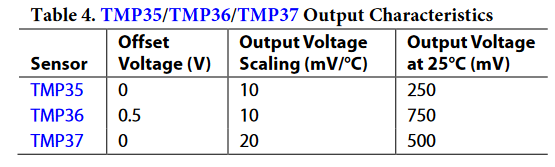
\includegraphics[width = 0.6\textwidth]{lab2images/tmp36_offset_documentation.png}}
\end{center}

For the Thermistor, we utilize \textbf{Eq.(5)} to convert the output voltage into degrees Celsius. By gathering the Thermistor's resistance along with the temperature in each environment we can set up and solve a system of linear equations as shown below:
\begin{center}
    $\begin{bmatrix}
        1 & ln(R_{T_{1}}) & (ln(R_{T_{1}}))^{3}\\[3pt]
        1 & ln(R_{T_{2}}) & (ln(R_{T_{2}}))^{3}\\[3pt]
        1 & ln(R_{T_{3}}) & (ln(R_{T_{3}}))^{3}
    \end{bmatrix}
    \cdot
    \begin{bmatrix}
        A\\[3pt]
        B\\[3pt]
        C
    \end{bmatrix}
    = 
    \begin{bmatrix}
        \frac{1}{T_{1}+273.15}\\[3pt]
            
        \frac{1}{T_{2}+273.15}\\[3pt]
        
        \frac{1}{T_{3}+273.15}
    \end{bmatrix}$
\end{center}

\subsubsection*{Mean Temperature in Laboratory w/ Confidence Interval}
Calculation of the mean temperature with confidence interval of $\gamma = 95\%$ was implemented through MATLAB as shown below:
\begin{lstlisting}[style=Matlab-editor]
% Confidence Interval in Laboratory
gamma = 0.95; %95 percent confidence

Fz = 0.5*(1+gamma);

nu = Q-1; %DOF, where Q is the # of samples

p = (1-gamma)/2; %probability

tstat = tinv(p,nu); 

% (SAMPLE MEANS) Mean w/ Confidence Interval
avg_unc_thermistor = [mean(thermistordata) 
                     tstat*std(thermistordata)/sqrt(Q)];

avg_unc_IC = [mean(ICdata) 
             tstat*std(ICdata)/sqrt(Q)];

avg_unc_thermocouple = [mean(thermocoupledata)  
                       tstat*std(thermocoupledata)/sqrt(Q)];
\end{lstlisting}

We define $F(z) = \frac{1}{2}(1+\gamma) = 0.9750$. The degrees of freedom (D.O.F.) $\nu = N - 1 = 59,999$ where $N=60,000$ samples. Set $P=\dfrac{1-\gamma}{2}=0.0250$. Using MATLAB function \textit{tinv}, we calculate the t-statistic to be $t_{stat} = -1.960$ or according to the \hyperlink{1}{t-distribution tables} this is also just $t_{stat}=1.960$.

Below are the average temperatures w/ the confidence interval for each of the three sensors:
\begin{itemize}
    \item Thermistor: \(1.1743 \pm 0.0001\; V \)
    \item IC/TMP36: \(20.8415 \pm 0.0038\; \degree C\)
    \item Thermocouple: \(21.6671 \pm 0.0005\; \degree C\)
\end{itemize}

For calibration, we had three different equations, one for each sensor. The thermistor's calibration equation was the Steinhart-Hart relation, the IC/TMP36 was a simple linear equation, and the thermocouple was a simple linear equation.

IC TMP36 Calibration:
\[
    T = a * V_{out} + b
\]
where $a = 100\; \degree C/V$ and $b = -50\; \degree C$.

Thermocouple Calibration:
\[
    T = a * V_{out} + b
\]

Thermistor Calibration:
\[
    T = \dfrac{1}{A + B\cdot ln(R_{T}) + C\cdot (ln(R_{T}))^{3}}
\]




\subsection{Part 2: Hot and Cold Water}

\subsubsection{Part 2a: Hot Water} % Subsubsection 1



\subsubsection{Part 2b: Water Cooling} % Subsubsection 2


\subsubsection{Part 2c: Ice-Hot} % Subsubsection 3


\subsubsection{Part 2d: Quick Changes} % Subsubsection 4


\subsubsection{Part 2e: Sensor Repetition} % Subsubsection 5



\section{Results}
This section analyzes the results of our data for the three temperature sensors in each environment.

\begin{table}
    \centering
    \begin{tabular}{cccc}
         &  Ambient&  Hot& Cold\\
         True Temperature ()&  &  & \\
         Voltage (V)&  &  & \\
 Resistance ()& & &\\
    \end{tabular}
    \caption{Caption}
    \label{tab:my_label}
\end{table}

\begin{figure}[H]
    \centering
    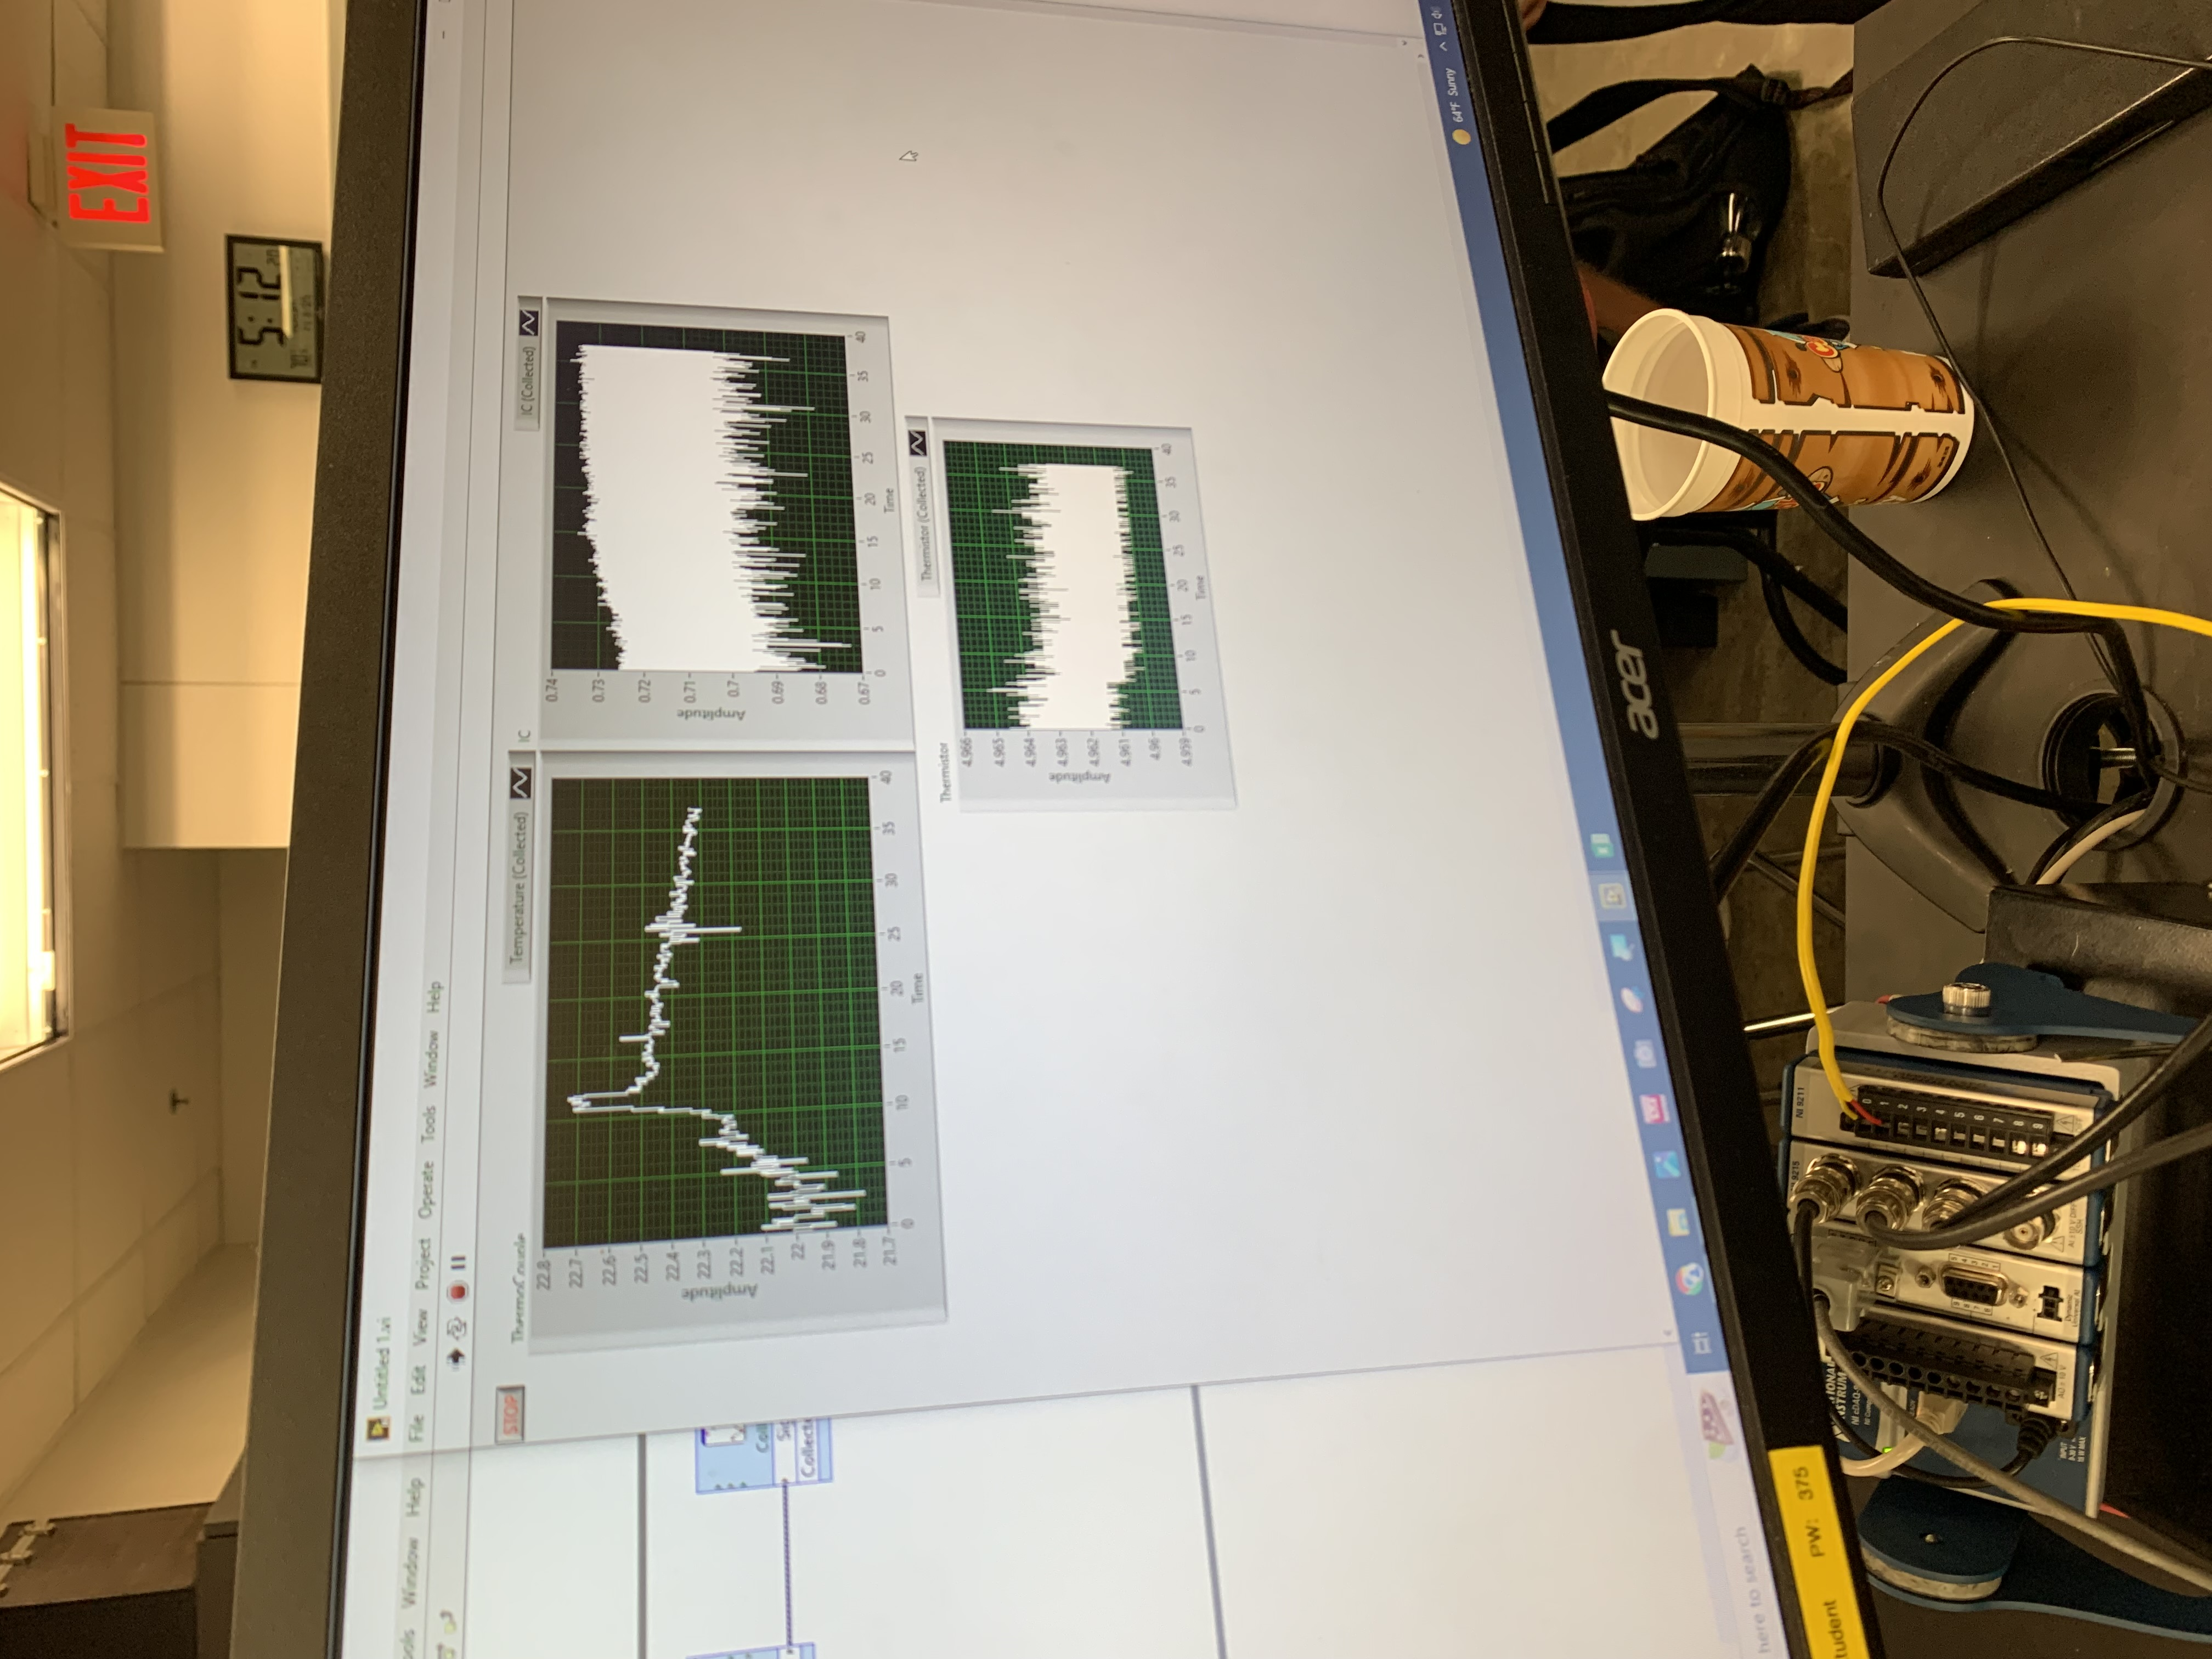
\includegraphics[width=0.5\textwidth, angle = -90]{lab2images/labview_plots.jpg}
    \caption{Plotting data on LabVIEW}
    \end{figure}
    
    \subsection{Part 1: Ambient Temperature}
    In Part 1 of the experiment we take measurements of the laboratory room temperature using each of the three sensors: thermocouple, thermistor, and IC TMP36. The data displayed below shows the temperature sensors at work for $1$ minute of sampling at $f_{s} = 1000\; s^{-1}$. This means $\Delta t_{s} = (f_{s}\cdot 60)^{-1} = 1.6667\times10^{-5}\; \text{minutes}$.
    
    \begin{figure}[H]
        \centering
        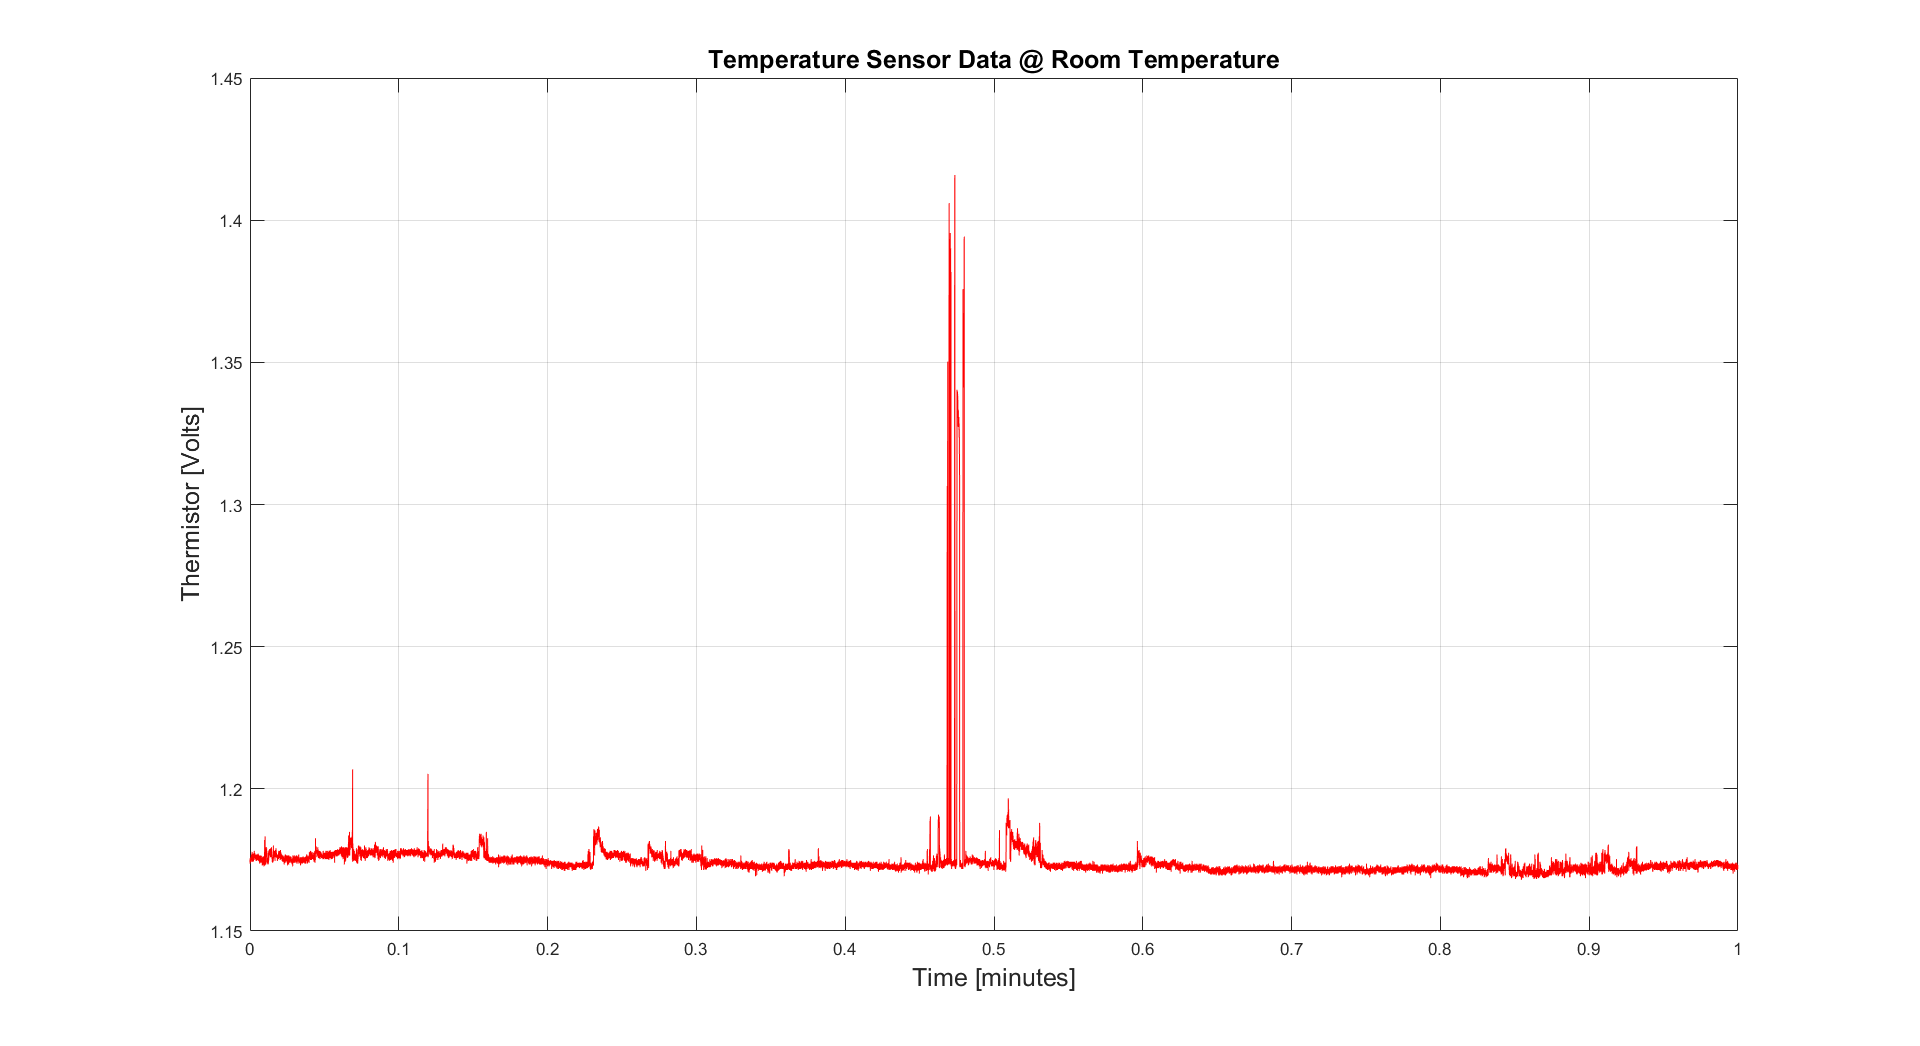
\includegraphics[width=0.655\textwidth]{lab2images/thermistor_volt_roomtemp_1min_plot.png}
        \caption{Thermistor at ambient temperature}
    \end{figure}
    
    \begin{figure}[H]
        \centering
        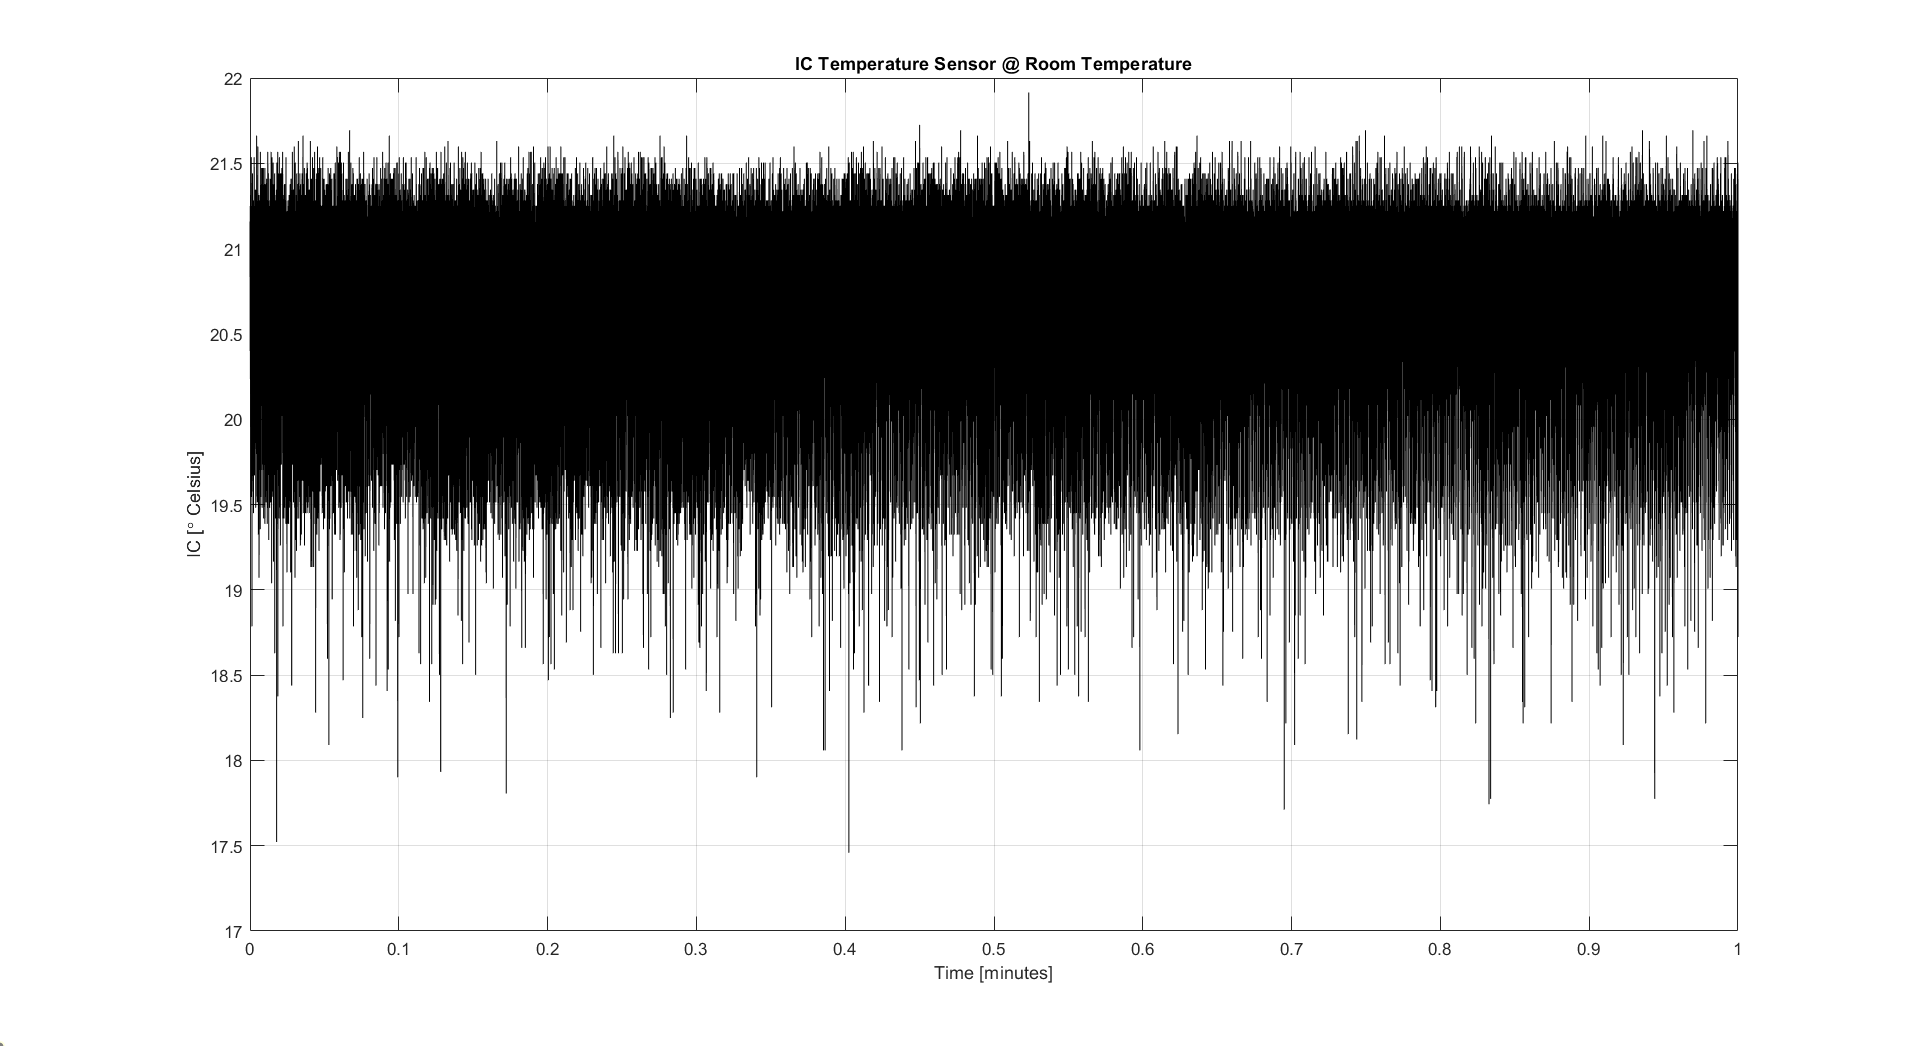
\includegraphics[width=0.655\textwidth]{lab2images/ICTMP36_roomtemp_1min_plot.png}
        \caption{IC TMP36 at ambient temperature}
    \end{figure}
    
    \begin{figure}[H]
        \centering
        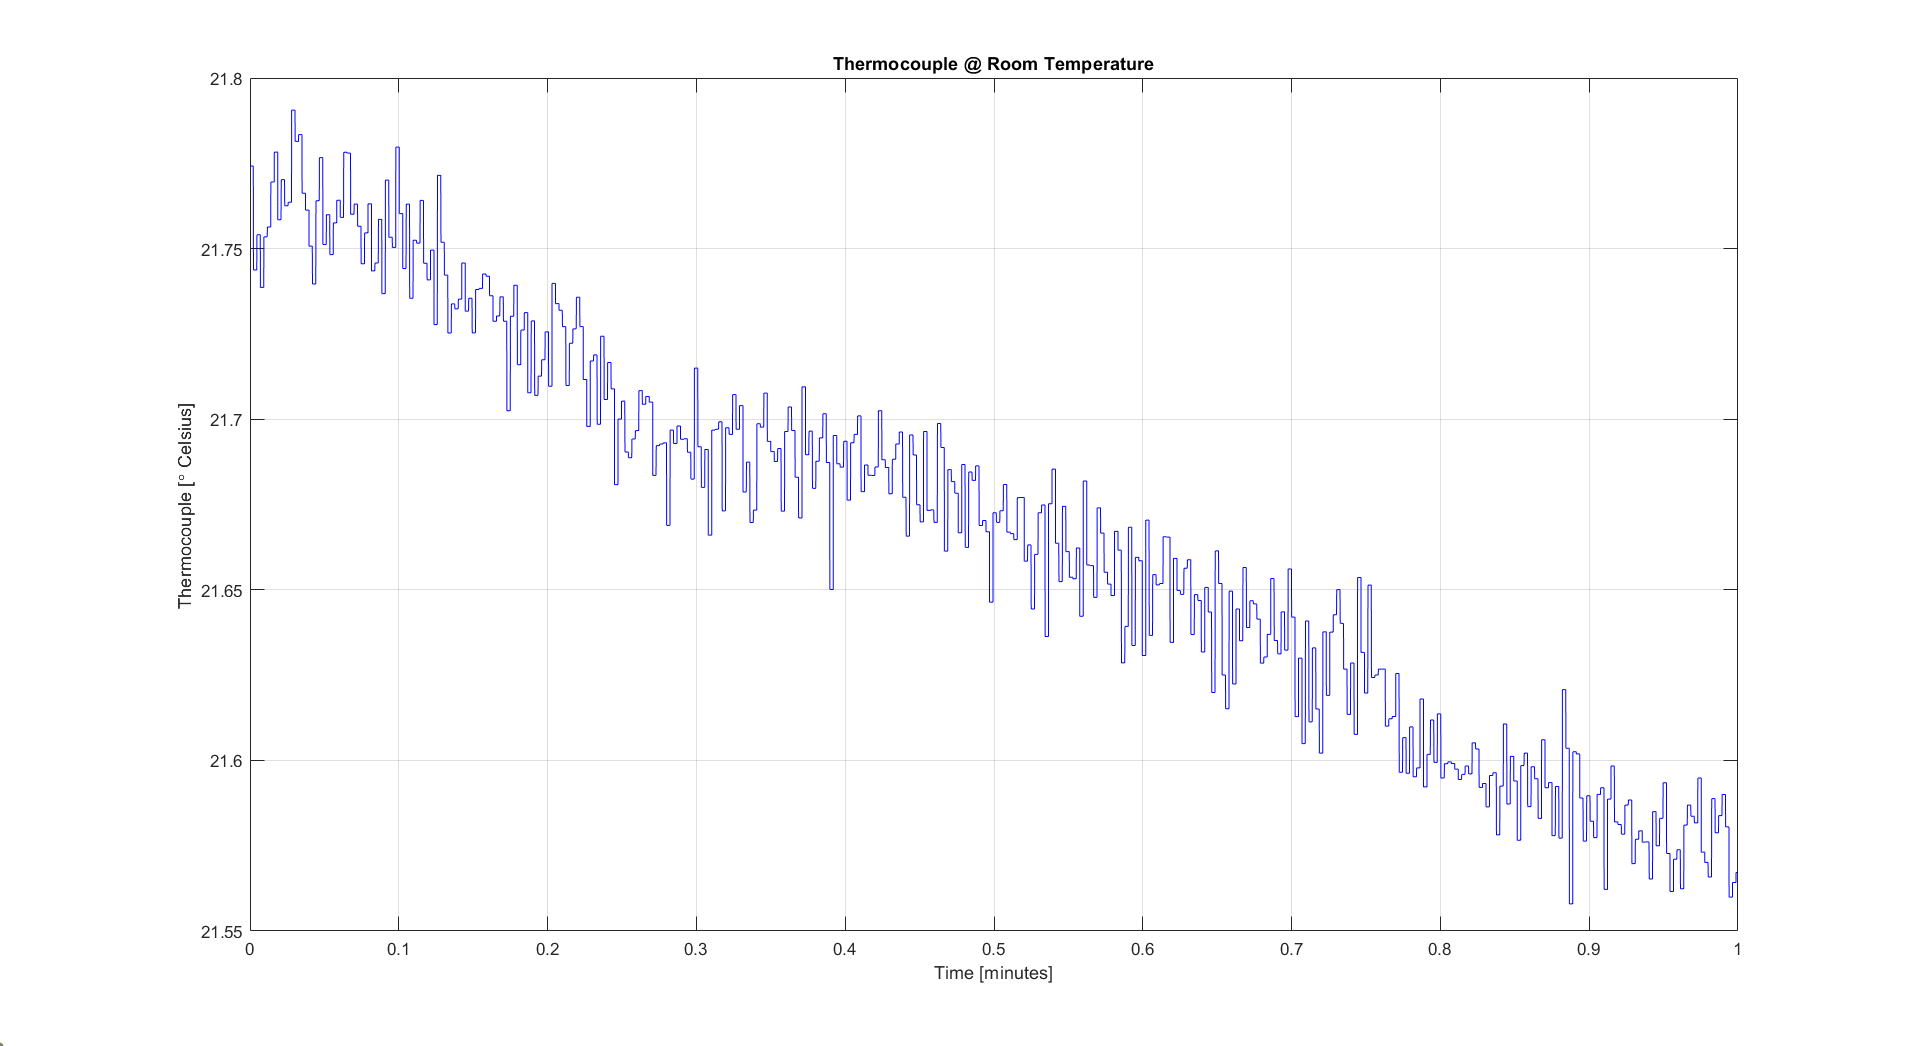
\includegraphics[width=0.655\textwidth]{lab2images/thermocouple_roomtemp_1min_plot.png}
        \caption{Thermocouple at ambient temperature}
    \end{figure}


    
    There are small spikes occurring around half of the period for the Thermistor's output. This disturbance could have been due to the Thermistor's sensitivity to very small changes in temperature, possibly due to slight movement (increased kinetic energy correlates to increased thermal energy).
    
    The TMP36 data appears similar to a white noise response for the entirety of the $1$ minute period with its large temperature interval. This shows the inaccuracy of the TMP36 when comparing to the other two sensors.
    
    Similar to the small change in the Thermistor's output, the Thermocouple sees small changes as it is decreasing to a steady-state. 

(Answer Observation Questions from Part 2)
QUESTIONS THAT GOTTA BE ANSWERED.
    a) time to reach steady state.  time constant of the sensor.  
    b) how long to cool to a safe, drinkable temp?
    c) how long to reach steady state.  is the time constant different than a?
    d) how long does it take to cool to ambient temp.  is this time constant different than a? 

% someone should make a table 


% use these to calculate A,B,C from steinhart-hart for calibrated output temp

The time constant, \(\tau\),  is defined as the time it takes for the system to change from its original state by 63\%.  % T(t)=(Tf=To)(1-exp(-t/tau))+To then find T at t=tau
Part 1 %For ambient temp
\begin{table}
    \centering
    \begin{tabular}{ccccc}
         &  Mean&  STD&  95\% confidence& Error\\
         Thermocouple&  &  &  & \\
         Thermistor&  &  &  & \\
         IC Sensor&  &  &  & \\
    \end{tabular}
    \caption{Caption}
    \label{tab:my_label}
\end{table}
    %add another column if needed?
    
%add graphs here of part a,b,c,d etc...

Part 2: %sudden changes in temp

\begin{table}
    \centering
    \begin{tabular}{cccccc}
         &  ambient to hot: sudden&  hot to cool: slow&  cold to hot: sudden&  hot to ambient: sudden& \\
         Initial Temp&  &  &  &  & \\
         Final Temp&  &  &  &  & \\
         Time Change From steady-state to steady-state&  &  &  &  & \\
         T at t=tau&  &  &  &  & \\
         time constant Tau&  &  &  &  & \\
    \end{tabular}
    \caption{Caption}
    \label{tab:sudden_temp}
\end{table}

\section{Conclusion}




\newpage
\thispagestyle{empty}  % Clear header/footer
\begin{center}
	\vspace*{\fill}
	{\Huge Appendices}
	\vspace*{\fill}
\end{center}

% Start appendices
\newpage
\begin{appendices}
\pagestyle{fancy}
\renewcommand{\thefigure}{A\arabic{figure}}
\setcounter{figure}{0}

\section*{Appendix: t-Distribution Tables}
\hypertarget{1}{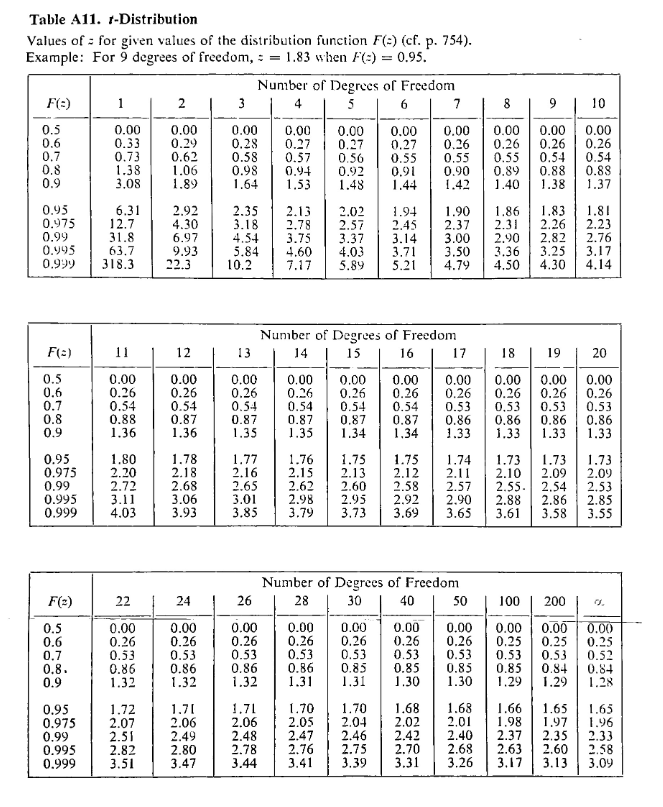
\includegraphics[width=0.95\textwidth]{t_distribution_Table_lecture3.png}}
\end{appendices}

\end{document}
